\chapter{Experimental results}
\label{cpt:experiments}

To evaluate Tribler's current situation and to validate our implementations are working correctly, experiments have been conducted.
In this chapter we elaborate on these experiments and discuss the results. 

\section{Tribler's I/O over the years}
As explained earlier, Tribler's I/O has been a problem for years.
To observe if and how the amount of I/O has changed over time, we have performed measurements on four \todo{change if needed} different versions of Tribler using iotop\footnote{\url{http://guichaz.free.fr/iotop/}}.
The versions and their release dates are depicted in Table~\ref{table:tribler_version_dates}.
The hardware used during this experiment can be found in Table \ref{table:tribler_idle} \todo{Change to VM 15.10 specs}.

As these measurements were never performed systematically, it is vital to perform these measurement now to observe if any changes have occurred between releases and document them.
This will provide valuable insight in Tribler's behaviour and the extent of the problem.
Moreover it will show us if the amount of I/O is being reduced since the creating of the ticker on GitHub.

\begin{table}[h]
	\centering
	\caption{The versions of Tribler and their release dates.}
	\label{table:tribler_version_dates}
	\begin{tabular}{|l|l|}
		\hline
		Tribler version & Release date \\ \hline
		6.3.5           &              \\ \hline
		6.4.3           &              \\ \hline
		6.5.2           &              \\ \hline
		6.6.0-exp1      &              \\ \hline
	\end{tabular}
\end{table}

\begin{table}[h]
	\centering
	\begin{tabular}{l|l}
		\textbf{Component} 	& \textbf{Specifications} \\ \hline
		Operating System   	& Ubuntu 16.04 LTS \\
		Python version		& 2.7.12 \\
		CPU					& Intel Core i5-2410M \\ 
		HDD					& Samsung 850 EVO 250GB  \\ 
		RAM					& 8 GB DDR3 1600MHz \\
	\end{tabular}
	\caption{Specifications of the setup used during the idle iotop measurement of Tribler 6.6.0-pre-exp.}
	\label{table:tribler_idle}
\end{table}

\begin{figure}[!h]
	\centering
	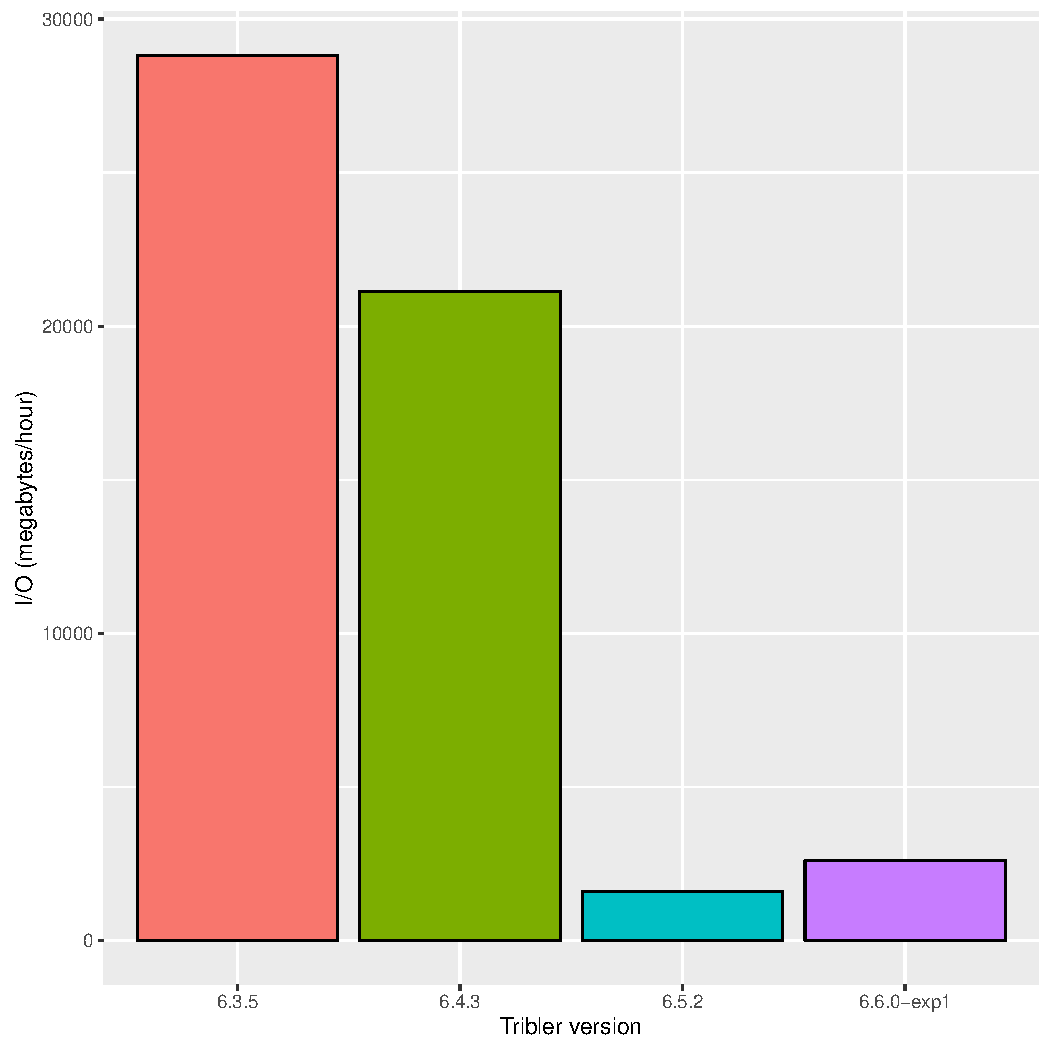
\includegraphics[width=\linewidth]{experimentation/images/io_history}
	\caption{The amount of I/O per version of Tribler.}
	\label{fig:io_history}
\end{figure} 

Each version of Tribler will run for one hour idle, using a clean state directory i.e. no prior knowledge of the network and its contents.
During the idle run, Tribler will start discovering peers and content such as channels and torrents, storing the obtained data in the database which gets flushed to disk.
Additionally, peers will start requesting data from this Tribler instance such as search and peer exchange requests, causing Tribler to read data from the database.
These read and writes operations will be monitored by iotop and the amounts automatically accumulated.
After one hour, the amount of read and write I/O is noted down and Tribler is shutdown.

The results of this experiment are visible in Figure~\ref{fig:io_history}.
From this figure we observe that Tribler's I/O has reduced significantly in version 6.5.2, yet is climbing again in the latest release due to the MultiChain feature added. 

Additionally, the numbers observed in this experiment are significantly higher than the numbers reported in the original ticket.
We believe the reason for this is due to the 100 mbit connection of the experiment machine, providing excellent connectability conditions. 
Secondly, the fact that it began with a clean state directory while running idle, provides ideal conditions for Tribler to spend most of its resources on discovering peers and content.

Finally, we observe that the total amount of I/O the latest version of Tribler is performing is 2598 MB/hour.
This shows the urgency of the I/O to become asynchronous and non-blocking.

\section{I/O breakdown}

\begin{table}[]
	\centering
	\caption{A breakdown of the functions called on StormDBManager.}
	\label{table:breakdown_tribler_idle}
	\begin{tabular}{|l|r|r|l|l|l|}
		\hline
		\textbf{Query}	& \textbf{Amount of calls} & \textbf{Total time (s)} & \textbf{Max}  & \textbf{Average} & \textbf{Min} \\ \hline
		fetchone	& 83036	& 3361.644 	& 0.81436	& 0.04048	& 0.00006 \\ \hline
		fetchall	& 2569	& 22.512	& 0.66344	& 0.00876	& 0.00007 \\ \hline
		execute		& 422	& 2.326  	& 0.20488	& 0.00551	& 0.00007 \\ \hline
		executemany	& 1		& 0.009 	& 0.00915 	& 0.00915	& 0.00915 \\ \hline
	\end{tabular}
\end{table}

To observe the individual components separately, we have created a breakdown of the database queries performed by Tribler and Dispersy.
We have run Tribler idle for one hour and tracked how many times each function in StormDBManager was called by either Dispersy or Tribler and how long it takes between scheduling the query the callback being invoked.
A breakdown of the functions is visible in Table~\ref{table:breakdown_tribler_idle}.
From this table we see that the \enquote{fetchone} function is being called the most, but what does this mean\todo{change and elaborate}

\section{Tribler's responsiveness}

To measure the performance gain of Tribler, we have conducted two sets of experiments where two instances of Tribler, one with the old implementation and one with the asynchronous version of Dispersy, are compared.

In the first experiment we have ran Tribler idle for one hour while querying the Twisted event loop every 100 milliseconds for delayed calls.
By doing so we can observe if certain tasks have been delayed past their set time of execution i.e. measure the latency in the system.

In the second experiment we have stress-tested Tribler's new API.
By requesting data from an endpoint at several rates per second, we can observe the throughput, response times, variance in these response times and throughput of Tribler.

\subsection{Measuring the latency of Tribler}

In this experiment we have compared two versions of Tribler, one with Dispersy having  blocking, synchronous I/O and one with Dispersy running StormDBManager and thus having non-blocking, asynchronous I/O.
Each instance of Tribler was run one hour idle where every 100 milliseconds the event loop of Twisted was queried for delayed calls.
By observing if delayed calls are past their set time of execution, we can measure the amount of latency in the system.

\subsection{Measuring the responsiveness of Tribler}



\section{Scalability}

If allchannel works, talk about scalability of nodes. \todo{todo}


